\documentclass[12pt,letterpaper]{article}
\usepackage{graphicx,textcomp}
\usepackage{natbib}
\usepackage{setspace}
\usepackage{fullpage}
\usepackage{color}
\usepackage[reqno]{amsmath}
\usepackage{amsthm}
\usepackage{fancyvrb}
\usepackage{amssymb,enumerate}
\usepackage[all]{xy}
\usepackage{endnotes}
\usepackage{lscape}
\newtheorem{com}{Comment}
\usepackage{float}
\usepackage{hyperref}
\newtheorem{lem} {Lemma}
\newtheorem{prop}{Proposition}
\newtheorem{thm}{Theorem}
\newtheorem{defn}{Definition}
\newtheorem{cor}{Corollary}
\newtheorem{obs}{Observation}
\usepackage[compact]{titlesec}
\usepackage{dcolumn}
\usepackage{tikz}
\usetikzlibrary{arrows}
\usepackage{multirow}
\usepackage{xcolor}
\newcolumntype{.}{D{.}{.}{-1}}
\newcolumntype{d}[1]{D{.}{.}{#1}}
\definecolor{light-gray}{gray}{0.65}
\usepackage{url}
\usepackage{listings}
\usepackage{color}

\definecolor{codegreen}{rgb}{0,0.6,0}
\definecolor{codegray}{rgb}{0.5,0.5,0.5}
\definecolor{codepurple}{rgb}{0.58,0,0.82}
\definecolor{backcolour}{rgb}{0.95,0.95,0.92}

\lstdefinestyle{mystyle}{
	backgroundcolor=\color{backcolour},   
	commentstyle=\color{codegreen},
	keywordstyle=\color{magenta},
	numberstyle=\tiny\color{codegray},
	stringstyle=\color{codepurple},
	basicstyle=\footnotesize,
	breakatwhitespace=false,         
	breaklines=true,                 
	captionpos=b,                    
	keepspaces=true,                 
	numbers=left,                    
	numbersep=5pt,                  
	showspaces=false,                
	showstringspaces=false,
	showtabs=false,                  
	tabsize=2
}
\lstset{style=mystyle}
\newcommand{\Sref}[1]{Section~\ref{#1}}
\newtheorem{hyp}{Hypothesis}

\title{Problem Set 2}
\date{\today}
\author{Kaley Burg}


\begin{document}
	\maketitle
	\section*{Instructions}
	\begin{itemize}
		\item Please show your work! You may lose points by simply writing in the answer. If the problem requires you to execute commands in \texttt{R}, please include the code you used to get your answers. Please also include the \texttt{.R} file that contains your code. If you are not sure if work needs to be shown for a particular problem, please ask.
		\item Your homework should be submitted electronically on GitHub in \texttt{.pdf} form.
		\item This problem set is due before 23:59 on Sunday February 18, 2024. No late assignments will be accepted.
	%	\item Total available points for this homework is 80.
	\end{itemize}

	
	%	\vspace{.25cm}
	
%\noindent In this problem set, you will run several regressions and create an add variable plot (see the lecture slides) in \texttt{R} using the \texttt{incumbents\_subset.csv} dataset. Include all of your code.

	\vspace{.25cm}
%\section*{Question 1} %(20 points)}
%\vspace{.25cm}
\noindent We're interested in what types of international environmental agreements or policies people support (\href{https://www.pnas.org/content/110/34/13763}{Bechtel and Scheve 2013)}. So, we asked 8,500 individuals whether they support a given policy, and for each participant, we vary the (1) number of countries that participate in the international agreement and (2) sanctions for not following the agreement. \\

\noindent Load in the data labeled \texttt{climateSupport.RData} on GitHub, which contains an observational study of 8,500 observations.

\begin{itemize}
	\item
	Response variable: 
	\begin{itemize}
		\item \texttt{choice}: 1 if the individual agreed with the policy; 0 if the individual did not support the policy
	\end{itemize}
	\item
	Explanatory variables: 
	\begin{itemize}
		\item
		\texttt{countries}: Number of participating countries [20 of 192; 80 of 192; 160 of 192]
		\item
		\texttt{sanctions}: Sanctions for missing emission reduction targets [None, 5\%, 15\%, and 20\% of the monthly household costs given 2\% GDP growth]
		
	\end{itemize}
	
\end{itemize}

\newpage
\noindent Please answer the following questions:

\begin{enumerate}
	\item
	Remember, we are interested in predicting the likelihood of an individual supporting a policy based on the number of countries participating and the possible sanctions for non-compliance.
	\begin{enumerate}
		\item [] Fit an additive model. Provide the summary output, the global null hypothesis, and $p$-value. Please describe the results and provide a conclusion.
		%\item
		%How many iterations did it take to find the maximum likelihood estimates?
	\end{enumerate}
	\textbf{My answer:}
	
	\begin{itemize}

	\item First I imported the dataset, changed the outcome variable to binary (0, 1). I used a table to ensure that this worked properly. Then I made the countries and sanctions variables into unordered variables to be able to use them as dummy variables in the regression. I also removed the spaces in the countries variable labels
	\item Then I ran the logistic regression using glm() and family = 'binomial', shown in the code below:
	\lstinputlisting[language=R, firstline=49, lastline=79]{PS2_KB_Final.R}
	
	
	\item \textbf{Here is the summary output:}
	
	
	\begin{table}[!htbp] \centering 
		\caption{Additive Model Summary} 
		\label{} 
		\begin{tabular}{@{\extracolsep{5pt}}lc} 
			\\[-1.8ex]\hline 
			\hline \\[-1.8ex] 
			& \multicolumn{1}{c}{\textit{Dependent variable:}} \\ 
			\cline{2-2} 
			\\[-1.8ex] & choice\_bin \\ 
			\hline \\[-1.8ex] 
			sanctions5\% & 0.192$^{***}$ \\ 
			& (0.062) \\ 
			& \\ 
			sanctions15\% & $-$0.133$^{**}$ \\ 
			& (0.062) \\ 
			& \\ 
			sanctions20\% & $-$0.304$^{***}$ \\ 
			& (0.062) \\ 
			& \\ 
			countries80of192 & 0.336$^{***}$ \\ 
			& (0.054) \\ 
			& \\ 
			countries160of192 & 0.648$^{***}$ \\ 
			& (0.054) \\ 
			& \\ 
			Constant & $-$0.273$^{***}$ \\ 
			& (0.054) \\ 
			& \\ 
			\hline \\[-1.8ex] 
			Observations & 8,500 \\ 
			Log Likelihood & $-$5,784.130 \\ 
			Akaike Inf. Crit. & 11,580.260 \\ 
			\hline 
			\hline \\[-1.8ex] 
			\textit{Note:}  & \multicolumn{1}{r}{$^{*}$p$<$0.1; $^{**}$p$<$0.05; $^{***}$p$<$0.01} \\ 
		\end{tabular} 
	\end{table} 
	

	\item The odd ratios are also as follows:
	
	\newpage
	\begin{table}[!htbp] \centering 
		\caption{Odd Ratios} 
		\label{} 
		\begin{tabular}{@{\extracolsep{5pt}} cccccc} 
			\\[-1.8ex]\hline 
			\hline \\[-1.8ex] 
			(Intercept) & sanctions5\% & sanctions15\% & sanctions20\% & countries80of192 & countries160of192 \\ 
			\hline \\[-1.8ex] 
			$0.761$ & $1.211$ & $0.875$ & $0.738$ & $1.400$ & $1.912$ \\ 
			\hline \\[-1.8ex] 
		\end{tabular} 
	\end{table} 
	
	\item these are calculated from this code:
	\lstinputlisting[language=R, firstline=229, lastline=229]{PS2_KB_Final.R}
	
	\item The probabilities can also be calculated using the plogis() function (to obtain the probability for a given log-odds value), shown here \textit{Note: the plogis function is used throughout this document for probability calculations. When calculating based on just one variable alone (country or sanctoin level) it is calculated using plogis($\beta$) whereas when it is used for predicted probabilities looking at both levels, it uses plogis(-($\beta_0 + \beta_1$)) This explains why it is used in both areas and obtains different numbers}:
	
		\lstinputlisting[language=R, firstline=249, lastline=249]{PS2_KB_Final.R}
	
	\item These probabilities are shown here:
	
	
	\begin{table}[!htbp] \centering 
		\caption{Probabilities} 
		\label{} 
		\begin{tabular}{@{\extracolsep{5pt}} cccccc} 
			\\[-1.8ex]\hline 
			\hline \\[-1.8ex] 
			(Intercept) & sanctions5\% & sanctions15\% & sanctions20\% & countries80of192 & countries160of192 \\ 
			\hline \\[-1.8ex] 
			$0.432$ & $0.548$ & $0.467$ & $0.425$ & $0.583$ & $0.657$ \\ 
			\hline \\[-1.8ex] 
		\end{tabular} 
	\end{table} 
	
\item \textbf{The global null and alternative hypotheses are as follows:}
\[
\begin{aligned}
	H_0 &: \text{ All slopes are equal to } 0 \\
	H_a &: \text{ At least one slope is not equal to } 0
\end{aligned}
\]

	\item We can test this hypothesis using an ANOVA, shown here:
	\lstinputlisting[language=R, firstline=86, lastline=90]{PS2_KB_Final.R}
	\end{itemize}
	
\begin{table}[!htbp] \centering 
	\caption{ANOVA Results} 
	\label{} 
	\begin{tabular}{@{\extracolsep{5pt}} cccccc} 
		\\[-1.8ex]\hline 
		\hline \\[-1.8ex] 
		& Resid. Df & Resid. Dev & Df & Deviance & Pr(\textgreater Chi) \\ 
		\hline \\[-1.8ex] 
		1 & $8,499$ & $11,783.410$ & $$ & $$ & $$ \\ 
		2 & $8,494$ & $11,568.260$ & $5$ & $215.150$ & $< 2.2e-16^{***}$ \\ 
		\hline \\[-1.8ex] 
		\textit{Note:}  & \multicolumn{1}{r}{$^{*}$p$<$0.1; $^{**}$p$<$0.05; $^{***}$p$<$0.01} \\ 
	\end{tabular} 
\end{table} 

	
	\begin{itemize}
		\item \textbf{Interpretation of results and conclusions:}
	\item Here is the results written out as a logistic regression equation 

\begin{center}
	\begin{align*}
		\text{logit}[P(Y_i = 1|X_i)] = & 0.192 \times \text{sanctions5\%} \\
		& - 0.133 \times \text{sanctions15\%} \\
		& - 0.304 \times \text{sanctions20\%} \\
		& + 0.336 \times \text{countries80of192} \\
		& + 0.648 \times \text{countries160of192} \\
		& - 0.273 \times \text{Constant}
	\end{align*}
\end{center}

	\item \textbf{Interpretation of coefficients}
	\item \textbf{Intercept Log Odds Interpretation:} When 20 countries participate in the international agreements and there are no sanctions for missing emission reduction targets, then on average the log odds of an individual agreeing with the policy is \textbf{-0.273} This is a statistically significant relationship.
		\begin{itemize}

			\item \textbf{Intercept Odds Ratio Interpretation:} Furthermore, the baseline odds ratio can be represented as $e^{\hat{\beta}_0} = e^{-0.273} = 0.7613211$ meaning that 0.76 is the estimated baseline odds that an individual supports the policy
			\item Interpretation of this results means that on average, people do not support the policy
			\item 0.761 indicates that the odds of an individual supporting the policy are approximately 0.761 times lower than the odds of an individual not supporting it.
			\item \textbf{Intercept Probability Interpretation:} Furthermore, the baseline probability of supporting the policy is 0.432.
		\end{itemize}
	\item \textbf{Log Odds Interpretation:} A change from no sanctions to a 5\% sanction is associated, on average, with a \textbf{0.192} increase in the log odds of an individual agreeing with the policy, holding the number of countries participating constant. This is a statistically significant relationship.
		\begin{itemize}
			\item \textbf{Odds Ratio Interpretation:} A change from no sanctions to a 5\% sanction increases the odds of supporting the policy by a multiplicative factor of 1.211; it
			increases the odds by $\approx$ 21.1\%, controlling for country participation.
				\item \textbf{Probabilities Interpretation:} A change from no sanctions to 5\% sanctions is associated with an, on average, 0.548 increase in the probability of supporting the policy, controlling for country participation. 
		\end{itemize}
	\item \textbf{Log Odds Interpretation:} A change from a 5\% sanction to a 15\% sanction is associated, on average, with a \textbf{0.133} decrease in the log odds of an individual agreeing with the policy, holding the number of countries participating constant. This is a statistically significant relationship.
		\begin{itemize}
			\item \textbf{Odds Ratio Interpretation:} A change from a 5\% sanction to a 15\% sanction decreases the odds of supporting the policy by a multiplicative factor of 0.875; it
			decreases the odds by $\approx$ 12.5\%, controlling for country participation.
				\item \textbf{Probabilities Interpretation:} A change from no sanctions to 15\% sanctions is associated with an, on average, 0.467 decrease in the probability of supporting the policy, controlling for country participation. 
		\end{itemize}
	\item \textbf{Log Odds Interpretation:} A change from a 15\% sanction to a 20\% sanction is associated, on average, with a \textbf{0.304} decrease in the log odds of an individual agreeing with the policy, holding the number of countries participating constant. This is a statistically significant relationship.
		\begin{itemize}
			\item  \textbf{Odds Ratio Interpretation:}A change from a 15\% sanction to a 20\% sanction decreases the odds of supporting the policy by a multiplicative factor of 0.738; it
			decreases the odds by $\approx$ 26.2\%, controlling for country participation.
				\item \textbf{Probabilities Interpretation:} A change from no sanctions to 20\% sanctions is associated with an, on average, 0.425 decrease in the probability of supporting the policy, controlling for country participation. 
		\end{itemize}
	\item \textbf{Log Odds Interpretation:} A change from 20 of 192 to 80 of 192 countries participating in the international agreement is associated, on average, with a \textbf{0.336} increase in the log odds of an individual agreeing with the policy, holding sanctions constant. This is a statistically significant relationship.
		\begin{itemize}
			\item \textbf{Odds Ratio Interpretation:}A change from 20 of 192 to 80 of 192 countries participating in the international agreement increases the odds of supporting the policy by a multiplicative factor of 1.400; it increases the odds by $\approx$ 40.0\%, controlling for sanctions.
				\item \textbf{Probabilities Interpretation:} A change from 20 to 80 countries is associated with an, on average, 0.583 increase in the probability of supporting the policy, controlling for sanctions. 
		\end{itemize}
	\item \textbf{Log Odds Interpretation:} A change from 80 of 192 to 160 of 192 countries participating in the  international agreement is associated, on average, with a \textbf{0.648} increase in the log odds of an individual agreeing with the policy, holding sanctions constant. This is a statistically significant relationship.
		\begin{itemize}
			\item \textbf{Odds Ratio Interpretation:} A change from 80 of 192 to 160 of 192 countries participating in the  international agreement increases the odds of supporting the policy by a multiplicative factor of 1.912; it
			increases the odds by $\approx$ 91.2\%, controlling for sanctions.
				\item \textbf{Probabilities Interpretation:} A change from 20 to 160 countries is associated with an, on average, 0.657 increase in the probability of supporting the policy, controlling for sanctions. 
		\end{itemize}
	
	\item \textbf{Interpretation of ANOVA}
	\item Since the p value is below a significance level of $\alpha$ = 0.05, this indicates that there is sufficient evidence to reject the global null hypothesis which states that all of the $\beta$ values are equal to 0. 

\end{itemize}
	
	
	
	
	
	
	
	
	
	
	
	\item
	If any of the explanatory variables are significant in this model, then:
	\begin{enumerate}
		\item
		For the policy in which nearly all countries participate [160 of 192], how does increasing sanctions from 5\% to 15\% change the odds that an individual will support the policy? (Interpretation of a coefficient)
		
		
		\begin{itemize}
			\item There a few different ways to solve this problem. First, the reference category in the regression can simply be set to the 5\% category. The code is shown here and the results are on the next page:
		\item \lstinputlisting[language=R, firstline=121, lastline=128]{PS2_KB_Final.R}
			
				\newpage
			
		\begin{table}[!htbp] \centering 
			\caption{} 
			\label{} 
			
		
			\begin{tabular}{@{\extracolsep{5pt}}lc} 
				\\[-1.8ex]\hline 
				\hline \\[-1.8ex] 
				& \multicolumn{1}{c}{\textit{Dependent variable:}} \\ 
				\cline{2-2} 
				\\[-1.8ex] & choice\_bin \\ 
				\hline \\[-1.8ex] 
				sanctionstestNone & $-$0.192$^{***}$ \\ 
				& (0.062) \\ 
				& \\ 
				sanctionstest15\% & $-$0.325$^{***}$ \\ 
				& (0.062) \\ 
				& \\ 
				sanctionstest20\% & $-$0.495$^{***}$ \\ 
				& (0.062) \\ 
				& \\ 
				countries80of192 & 0.336$^{***}$ \\ 
				& (0.054) \\ 
				& \\ 
				countries160of192 & 0.648$^{***}$ \\ 
				& (0.054) \\ 
				& \\ 
				Constant & $-$0.081 \\ 
				& (0.053) \\ 
				& \\ 
				\hline \\[-1.8ex] 
				Observations & 8,500 \\ 
				Log Likelihood & $-$5,784.130 \\ 
				Akaike Inf. Crit. & 11,580.260 \\ 
				\hline 
				\hline \\[-1.8ex] 
				\textit{Note:}  & \multicolumn{1}{r}{$^{*}$p$<$0.1; $^{**}$p$<$0.05; $^{***}$p$<$0.01} \\ 
			\end{tabular} 
		\end{table} 
		
		\item We can see that the change in sanctions from 5\% to 15\% is associated with a 0.32510 decrease in the log odds of supporting the policy
			\begin{itemize}
				\item Therefore, a change from 5 to 15\% sanctions in which nearly all countries are participating in the  international agreement decreases the odds of supporting the policy by a multiplicative factor of 0.722; it decreases the odds by $\approx$ 27.8\%. This is calculated, like before by performing $e^{-0.32510}$ or exp(-0.32510) in R to get the odds ratio from the log odds.
				\item Similar to the other problem, we can use the plogis() function to obtain the probability for a given log-odds value and we get a value of 0.4194333. This means that the estimated probability of supporting the policy when sanctions are set to 15\% (compared to 5\%) is approximately 42\%
				
			\end{itemize}
		\item It is also important to note that since this is an additive model, the change between 5 and 15\% sanctions is the same across all levels of country participation, as the slopes by country participation level are made equivalent.
		\item This can also be solved by hand when the reference category is set to "None" as follows:
		


\begin{align*}
	\text{SanctionsNone} + \beta_1 &= 0.19186 \\
	\text{SanctionsNone} + \beta_2 &= 0.13325 \\
\end{align*}

\begin{align*}
	(\text{SanctionsNone} + \beta_1 &= 0.19186) \\
	- (\text{SanctionsNone} + \beta_2 &= 0.13325) \\
	&= \beta_1 + \beta_2 = 0.19186 + 0.13325
\end{align*}

\begin{align*}
	\beta_1 - \beta_2 &= 0.32511 \\
	\smash{\begin{array}[t]{@{}c@{}}-\end{array}} \beta_2 - \beta_1 &= -0.32511
\end{align*}


\item As shown above, we get approximately the same answer as if we change the reference category




















		\end{itemize}
%		\item
%		For the policy in which very few countries participate [20 of 192], how does increasing sanctions from 5\% to 15\% change the odds that an individual will support the policy? (Interpretation of a coefficient)
		\item
		What is the estimated probability that an individual will support a policy if there are 80 of 192 countries participating with no sanctions?
		\begin{itemize}
		\item To find a predicted probability, we can use this equation:
		\[
		P(Y_i = 1 | X_i) = \frac{\exp(\beta_0 + \beta_1 x_i)}{1 + \exp(\beta_0 + \beta_1 x_i)}
		\]
		
		\item Using the $\beta$ coefficient associated with 80 of 192 countries participating and sanctions held at their reference level of "None," then we can plug in the values to get this equation:
		
		\[
		\frac{1}{1 + \exp\left(-(-0.27266 + 0.33636)\right)}
		\]
		
		\item This simplifies to 0.5159191
		\item Therefore, the estimated probability of an individual supporting the policy when 80 of 192 countries participate and there are no sanctions is \textbf{0.5159191} or 51.59\%.
		
		\item This could also be solved in R using the plogis() function
		\item \lstinputlisting[language=R, firstline=144, lastline=144]{PS2_KB_Final.R}
		
		\vspace{0.1cm}
		\item Additionally, we can use this function along with code adapted from the lecture slides to plot the predicted probabilities. The code for this is:
		\item \lstinputlisting[language=R, firstline=156, lastline=167]{PS2_KB_Final.R}
		
	 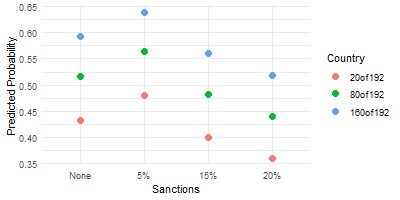
\includegraphics[width=0.8\textwidth]{mod_predprobs.png}
		
		\item Then, using this list of predicted values we can subset by sanctions set to None and countries set to 80 of 192. The code is as follows:
		\item \lstinputlisting[language=R, firstline=172, lastline=177]{PS2_KB_Final.R}
		\item This returns these values:
		
		\newpage
\begin{table}[htbp]
	\centering
	\caption{Predicted Probabilities - Additive Model}
	\label{tab:mytable}
	\begin{tabular}{|l|l|l|}
		\hline
		\textbf{Country Level} & \textbf{Sanctions} & \textbf{Probabilities} \\
		\hline
		80of192 & 15\% & 0.4826196 \\
		160of192 & 15\% & 0.5603146 \\
		160of192 & None & 0.5928323 \\
		160of192 & 5\% & 0.6381958 \\
		20of192 & 15\% & 0.3998931 \\
		80of192 & 20\% & 0.4403193 \\
		160of192 & 20\% & 0.5180228 \\
		20of192 & 5\% & 0.4798090 \\
		80of192 & 5\% & 0.5635428 \\
		\colorbox{yellow}{80of192} & \colorbox{yellow}{None} & \colorbox{yellow}{0.5159191} \\
		20of192 & 20\% & 0.3598012 \\
		20of192 & None & 0.4322534 \\
		\hline
	\end{tabular}
\end{table}
		
		\item We can see here that we get the same predicted value of 0.52
		
		\end{itemize} 
		\item
		Would the answers to 2a and 2b potentially change if we included the interaction term in this model? Why? 
		
		
		
		\begin{itemize}
			\item Yes, the answers to 2a and 2b would potentially change if we included an interaction term. This is because with an interaction term, the slopes are not necessarily equal across each of the variables.
			\item For example, in 2a, the change from 5 to 15\% sanctions is the same across all levels of country participation as we are modeling it to not vary along with country participation. Therefore, including an interaction term would potentially change this.
			
			\item We can see this when we run the interactive model:
			\item \lstinputlisting[language=R, firstline=186, lastline=189]{PS2_KB_Final.R}
			
 
			\begin{table} \centering 
				\caption{Interactive Logistic Regression Model} 
				\label{} 
				\begin{tabular}{@{\extracolsep{5pt}}lc} 
					\\[-1.8ex]\hline 
					\hline \\[-1.8ex] 
					& \multicolumn{1}{c}{\textit{Dependent variable:}} \\ 
					\cline{2-2} 
					\\[-1.8ex] & choice\_bin \\ 
					\hline \\[-1.8ex] 
					sanctions5\% & 0.122 \\ 
					& (0.105) \\ 
					& \\ 
					sanctions15\% & $-$0.097 \\ 
					& (0.108) \\ 
					& \\ 
					sanctions20\% & $-$0.253$^{**}$ \\ 
					& (0.108) \\ 
					& \\ 
					countries80of192 & 0.376$^{***}$ \\ 
					& (0.106) \\ 
					& \\ 
					countries160of192 & 0.613$^{***}$ \\ 
					& (0.108) \\ 
					& \\ 
					sanctions5\%:countries80of192 & 0.095 \\ 
					& (0.152) \\ 
					& \\ 
					sanctions15\%:countries80of192 & $-$0.052 \\ 
					& (0.152) \\ 
					& \\ 
					sanctions20\%:countries80of192 & $-$0.197 \\ 
					& (0.151) \\ 
					& \\ 
					sanctions5\%:countries160of192 & 0.130 \\ 
					& (0.151) \\ 
					& \\ 
					sanctions15\%:countries160of192 & $-$0.052 \\ 
					& (0.153) \\ 
					& \\ 
					sanctions20\%:countries160of192 & 0.057 \\ 
					& (0.154) \\ 
					& \\ 
					Constant & $-$0.275$^{***}$ \\ 
					& (0.075) \\ 
					& \\ 
					\hline \\[-1.8ex] 
					Observations & 8,500 \\ 
					Log Likelihood & $-$5,780.983 \\ 
					Akaike Inf. Crit. & 11,585.970 \\ 
					\hline 
					\hline \\[-1.8ex] 
					\textit{Note:}  & \multicolumn{1}{r}{$^{*}$p$<$0.1; $^{**}$p$<$0.05; $^{***}$p$<$0.01} \\ 
				\end{tabular} 
			\end{table} 
			
			\newpage
			\item Given the change in $\beta$ values, we can see that the associated change between 5 and 15\% sanctions for 160 of 192 countries participating would be associated with a -0.182 change in log odds of support for the policy (a decrease in odds by a multiplicative factor of 0.8336013)
			\item This is in comparison to without the additive model (change in log odds of -0.32510)
			\vspace{0.2cm}
			\item For 2c, the predicted values also are not guaranteed to have the same slopes. This is best demonstrated visually:
			\newline
			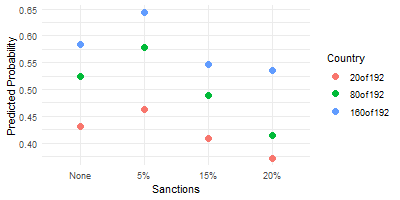
\includegraphics[width=0.8\textwidth]{modint_predprobs.png}
			\item We can see that the connections between points of the same country level have different slopes than that of the earlier plot. Therefore, the predicted values would change if we use an interactive model.
			\item This can also be demonstrated with the same code as above
			\lstinputlisting[language=R, firstline=207, lastline=212]{PS2_KB_Final.R}
			\item The results are included in the next page
		
		
\newpage
\begin{table}[htbp]
	\centering
	\caption{Predicted Probabilities - Interactive Model}
	\label{tab:mytable}
	\begin{tabular}{|l|l|l|}
		\hline
		\textbf{Country} & \textbf{Sanctions} & \textbf{Probability} \\
		\hline
			80of192 & 15\% & 0.4879433 \\
			160of192 & 15\% & 0.5472222 \\
			160of192 & None & 0.5836972 \\
			160of192 & 5\% & 0.6433289 \\
			20of192 & 15\% & 0.4081633 \\
			80of192 & 20\% & 0.4136546 \\
			160of192 & 20\% & 0.5355030 \\
			20of192 & 5\% & 0.4618474 \\
			80of192 & 5\% & 0.5786963 \\
			\colorbox{yellow}{80of192} & 	\colorbox{yellow}{None} & 	\colorbox{yellow}{0.5252101} \\
			20of192 & 20\% & 0.3711485 \\
			20of192 & None & 0.4317549 \\
			\hline
		\end{tabular}
	\end{table}
	
	\item We can see that the predicted value at 80 of 192 countries and no sanctions changes slightly from the previous table
		
		\end{itemize}
		
		
		
		
		\begin{itemize}
			\item Perform a test to see if including an interaction is appropriate.
				\begin{itemize}
					\item This can be tested using an ANOVA with the additive model and interactive model
					\lstinputlisting[language=R, firstline=220, lastline=220]{PS2_KB_Final.R}
					\item These are the ANOVA results:
					\begin{table}[!htbp] \centering 
						\caption{} 
						\label{} 
						\begin{tabular}{@{\extracolsep{5pt}}lccccc} 
							\\[-1.8ex]\hline 
							\hline \\[-1.8ex] 
							Statistic & \multicolumn{1}{c}{N} & \multicolumn{1}{c}{Mean} & \multicolumn{1}{c}{St. Dev.} & \multicolumn{1}{c}{Min} & \multicolumn{1}{c}{Max} \\ 
							\hline \\[-1.8ex] 
							Resid. Df & 2 & 8,491.000 & 4.243 & 8,488 & 8,494 \\ 
							Resid. Dev & 2 & 11,565.110 & 4.450 & 11,561.970 & 11,568.260 \\ 
							Df & 1 & 6.000 &  & 6 & 6 \\ 
							Deviance & 1 & 6.293 &  & 6.293 & 6.293 \\ 
							Pr(\textgreater Chi) & 1 & 0.391 &  & 0.391 & 0.391 \\ 
							\hline \\[-1.8ex] 
						\end{tabular} 
					\end{table} 
					\item We can see that the p value is 0.3912, so there is \textbf{not} sufficient evidence to able to reject the null hypothesis, meaning that the interaction is not appropriate.
				\end{itemize}
		\end{itemize}
	\end{enumerate}
	\end{enumerate}


\end{document}


